\section{Real-Data Training Curves}

\begin{figure*}[t]
\centering
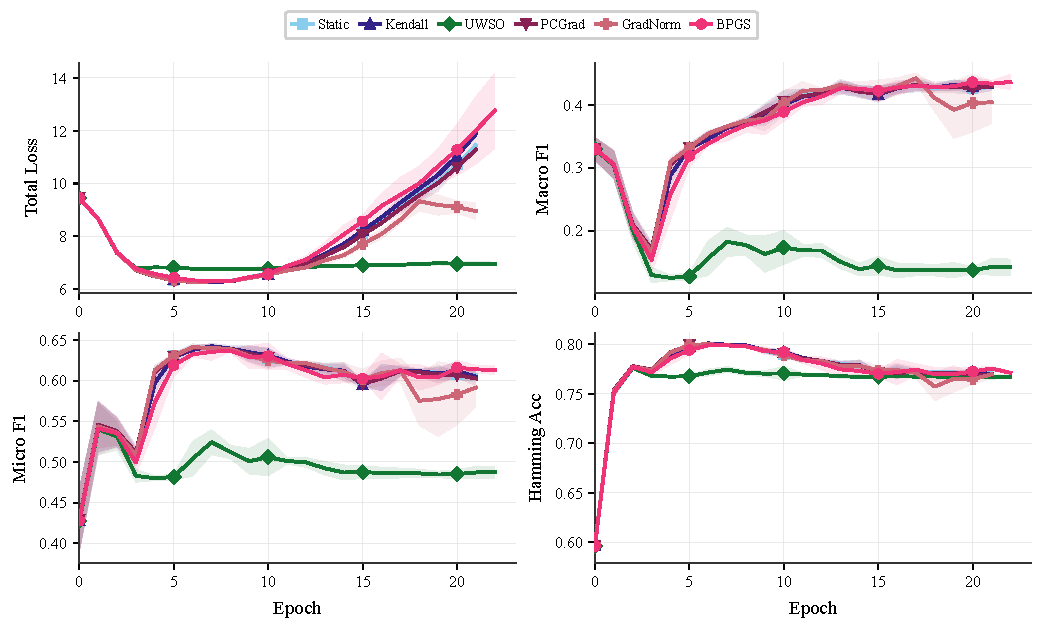
\includegraphics[width=\textwidth]{data/full_data/yeast/figures/pdf/yeast_training_curves.pdf}
\caption{Yeast training curves. BPGS tracks the strongest final micro-F1 and macro-F1 among the compared methods, while UWSO remains substantially weaker throughout training.}
\label{fig:appendix_yeast_curves}
\end{figure*}

\begin{figure*}[t]
\centering
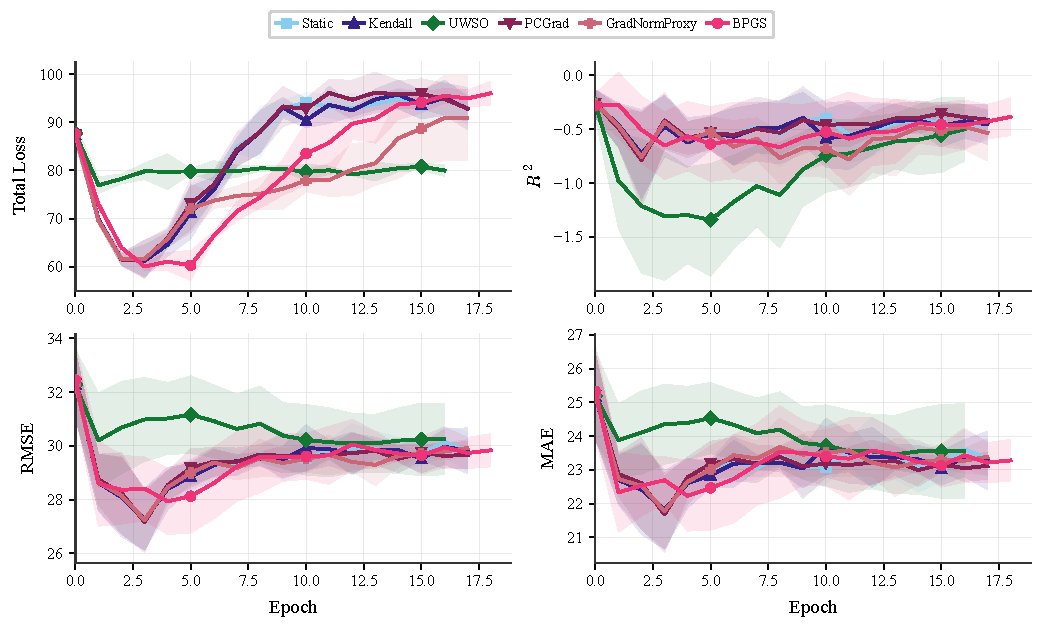
\includegraphics[width=\textwidth]{data/full_data/river_flow/figures/pdf/rf1_training_curves.pdf}
\caption{RF1 training curves. The methods remain closer than in the synthetic stress studies, which is consistent with the paper's claim that RF1 supports competitiveness rather than clear superiority.}
\label{fig:appendix_rf1_curves}
\end{figure*}
